% +------------------------------------------------------------------------+
% | CGAL Reference Manual:  snapRounding.tex
% +------------------------------------------------------------------------+
% | snap rounding of line segments
% |
% | 9.4.00   Eli Packer
% | 
\RCSdef{\snapRoundingRev}{$Revision$}
\RCSdefDate{\snapRoundingDate}{$Date$}
% +------------------------------------------------------------------------+

\ccParDims

% \usepackage{graphics, amssymb,epsfig}

\chapter{Line Segments Snap Rounding}
\label{chapterSnapRoundibg}
\ccChapterRelease{\snapRoundingRev. \ \snapRoundingDate}\\
\ccChapterAuthor{Eli Packer}
\newcommand{\reals}{{\rm I\!\hspace{-0.025em} R}}
\def\A{{\cal A}}
\def\S{{\cal S}}

% +------------------------------------------------------------------------+
\section{Introduction}
Snap rounding is a well known method for converting
arbitrary-precision arrangements of segments into a fixed-precision
representation. It is classified as a finite precision approximation 
technique. This package makes Snap Rounding of line segments in $\reals_2$.
It is based on the paper 'Snap Rounding Revisited' which provides a modification
to Snap Rounding named Iterated Snap Rounding. This package provides both
Iterated Snap Rounding and the usual Snap Rounding which is a private case.
For details we refer you to the article.

\begin{figure}
\begin{center}
\begin{ccTexOnly}
{\centering \resizebox*{0.4\textwidth}{0.15\textheight}%
 {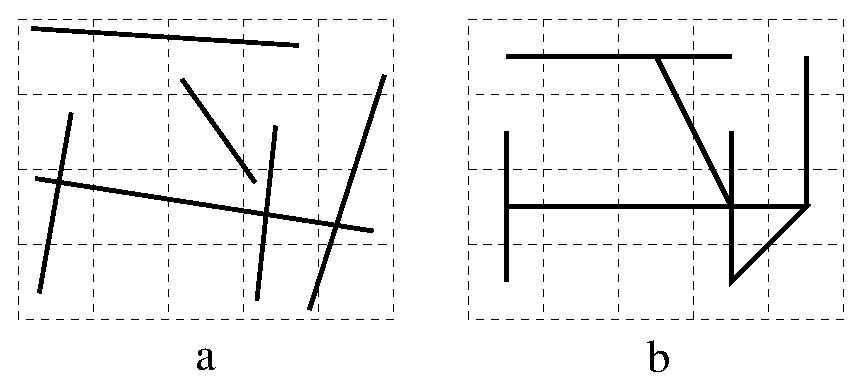
\includegraphics{sr1.ps}}
}
\end{ccTexOnly}
\caption{Snap rounding: before (a) and after (b).\label{fig:sr1}}
\begin{ccHtmlOnly}
<P>
<center><img border=0 src="./sr1.gif" alt=" ">
<!--
<br>
Snap rounding: before (a) and after (b).
-->
</center>
\end{ccHtmlOnly}
\end{center}
\end{figure}

Figure~\ref{fig:sr1} demonstrates a snap rounding output. 

\section{What is Snap Rounding/Iterated Snap Rounding}
Given a finite collection $\S$ of segments in the plane, the
arrangement of $\S$ denoted $\A(\S)$ is the subdivision of the plane
into vertices, edges, and faces induced by $\S$. %\cite{arrg-surveys}.
A {\it vertex\/} of the arrangement is either a segment endpoint or
the intersection of two segments. Given an arrangement of segments
whose vertices are represented with arbitrary-precision coordinates,
snap rounding (SR, for short) proceeds as follows.  We tile the plane
with a grid of unit squares, {\it pixels}, each centered at a point
with integer coordinates. A pixel is {\it hot\/} if it contains a
vertex of the arrangement. Each vertex of the arrangement is replaced
by the center of the hot pixel containing it and each edge $e$ is
replaced by the polygonal chain through the centers of the hot pixels
met by $e$, in the same order as they are met by $e$.

Since in a snap-rounded arrangement, the distance between a vertex and
a non-incident edge can be extremely small compared with the width of a
pixel in the grid used for rounding, this package provides, beside the
usual Snap Rounding, a modification of it, named Iterated Snap Rounding,
which makes the a vertex and a non-incident edge well separated.


% +========================================================================+
\section{Examples of Snap Rounding}
% +========================================================================+

The following example generates a snap rounding representation of an arrangement of four line segments
and a list of points which are the vertices of the resulting polylines.

% \ccIncludeExampleCode{../../examples/Snap_rounding/example.C}
\ccIncludeExampleCode{../../examples/Snap_rounding_2/example.C}
% +--------------------------------------------------------+

% EOF


